\documentclass[../notes.tex]{subfiles}

\pagestyle{main}
\renewcommand{\chaptermark}[1]{\markboth{\chaptername\ \thechapter\ (#1)}{}}
\setcounter{chapter}{7}

\begin{document}




\chapter{Crystal Structure and Surface Chemistry}
\section{X-Ray Diffraction Fundamentals}
\begin{itemize}
    \item \marginnote{5/16:}Final exam next Wednesday in class.
    \begin{itemize}
        \item 50 minutes.
        \item Questions like the midterm.
        \item We can bring our notes and textbook, but cannot search online.
        \begin{itemize}
            \item Can we bring notes on a computer, like mine, or do we have to print?
        \end{itemize}
        \item 1 computation problem.
        \item We will write answers on paper.
    \end{itemize}
    \item Review of last lecture.
    \item Tian goes through some examples of naming crystallographic planes from pictures of them intersecting a unit cell.
    \begin{itemize}
        \item The first example is a $111$ plane.
        \begin{itemize}
            \item If asked to identify a $111$ plane, it is enough to identify it as a $111$ plane; we do not have to identify it as a possible $222$ plane, too.
        \end{itemize}
        \item Consider a plane intersecting the \textbf{a}, \textbf{b}, and \textbf{c} axes at $a'=2a/5$, $b'=b/2$, and $c'=c/5$, respectively.
        \begin{itemize}
            \item Then $h=\frac{5}{2}$, $k=2$, and $l=5$.
            \item An easier way to show this, however, is with $h=5$, $k=4$, and $l=10$. Aren't these planes spaced twice as close together, though?
        \end{itemize}
        \item Consider a plane intersecting the \textbf{a}, \textbf{b}, and \textbf{c} axes at $a'=a/2$, $b'=b/2$, and $c'=-c/4$, respectively.
        \begin{itemize}
            \item A convenient point to use as the origin in this case is the upper-left corner.
            \item Thus, the plane is $(2,2,-4)$.
            \item The question of could we denote the plane by $(1,1,-2)$: These two sets of planes are parallel, but the spacing of $(1,1,-2)$ would skip every plane like $(2,2,-4)$. Thus, we need $(2,2,-4)$ for the spacing.
        \end{itemize}
    \end{itemize}
    \item Rules.
    \begin{enumerate}
        \item If you see a fraction, convert to integers.
        \item But do not reduce a ratio.
    \end{enumerate}
    \item The fundamentals of X-ray diffraction.
    \begin{figure}[H]
        \centering
        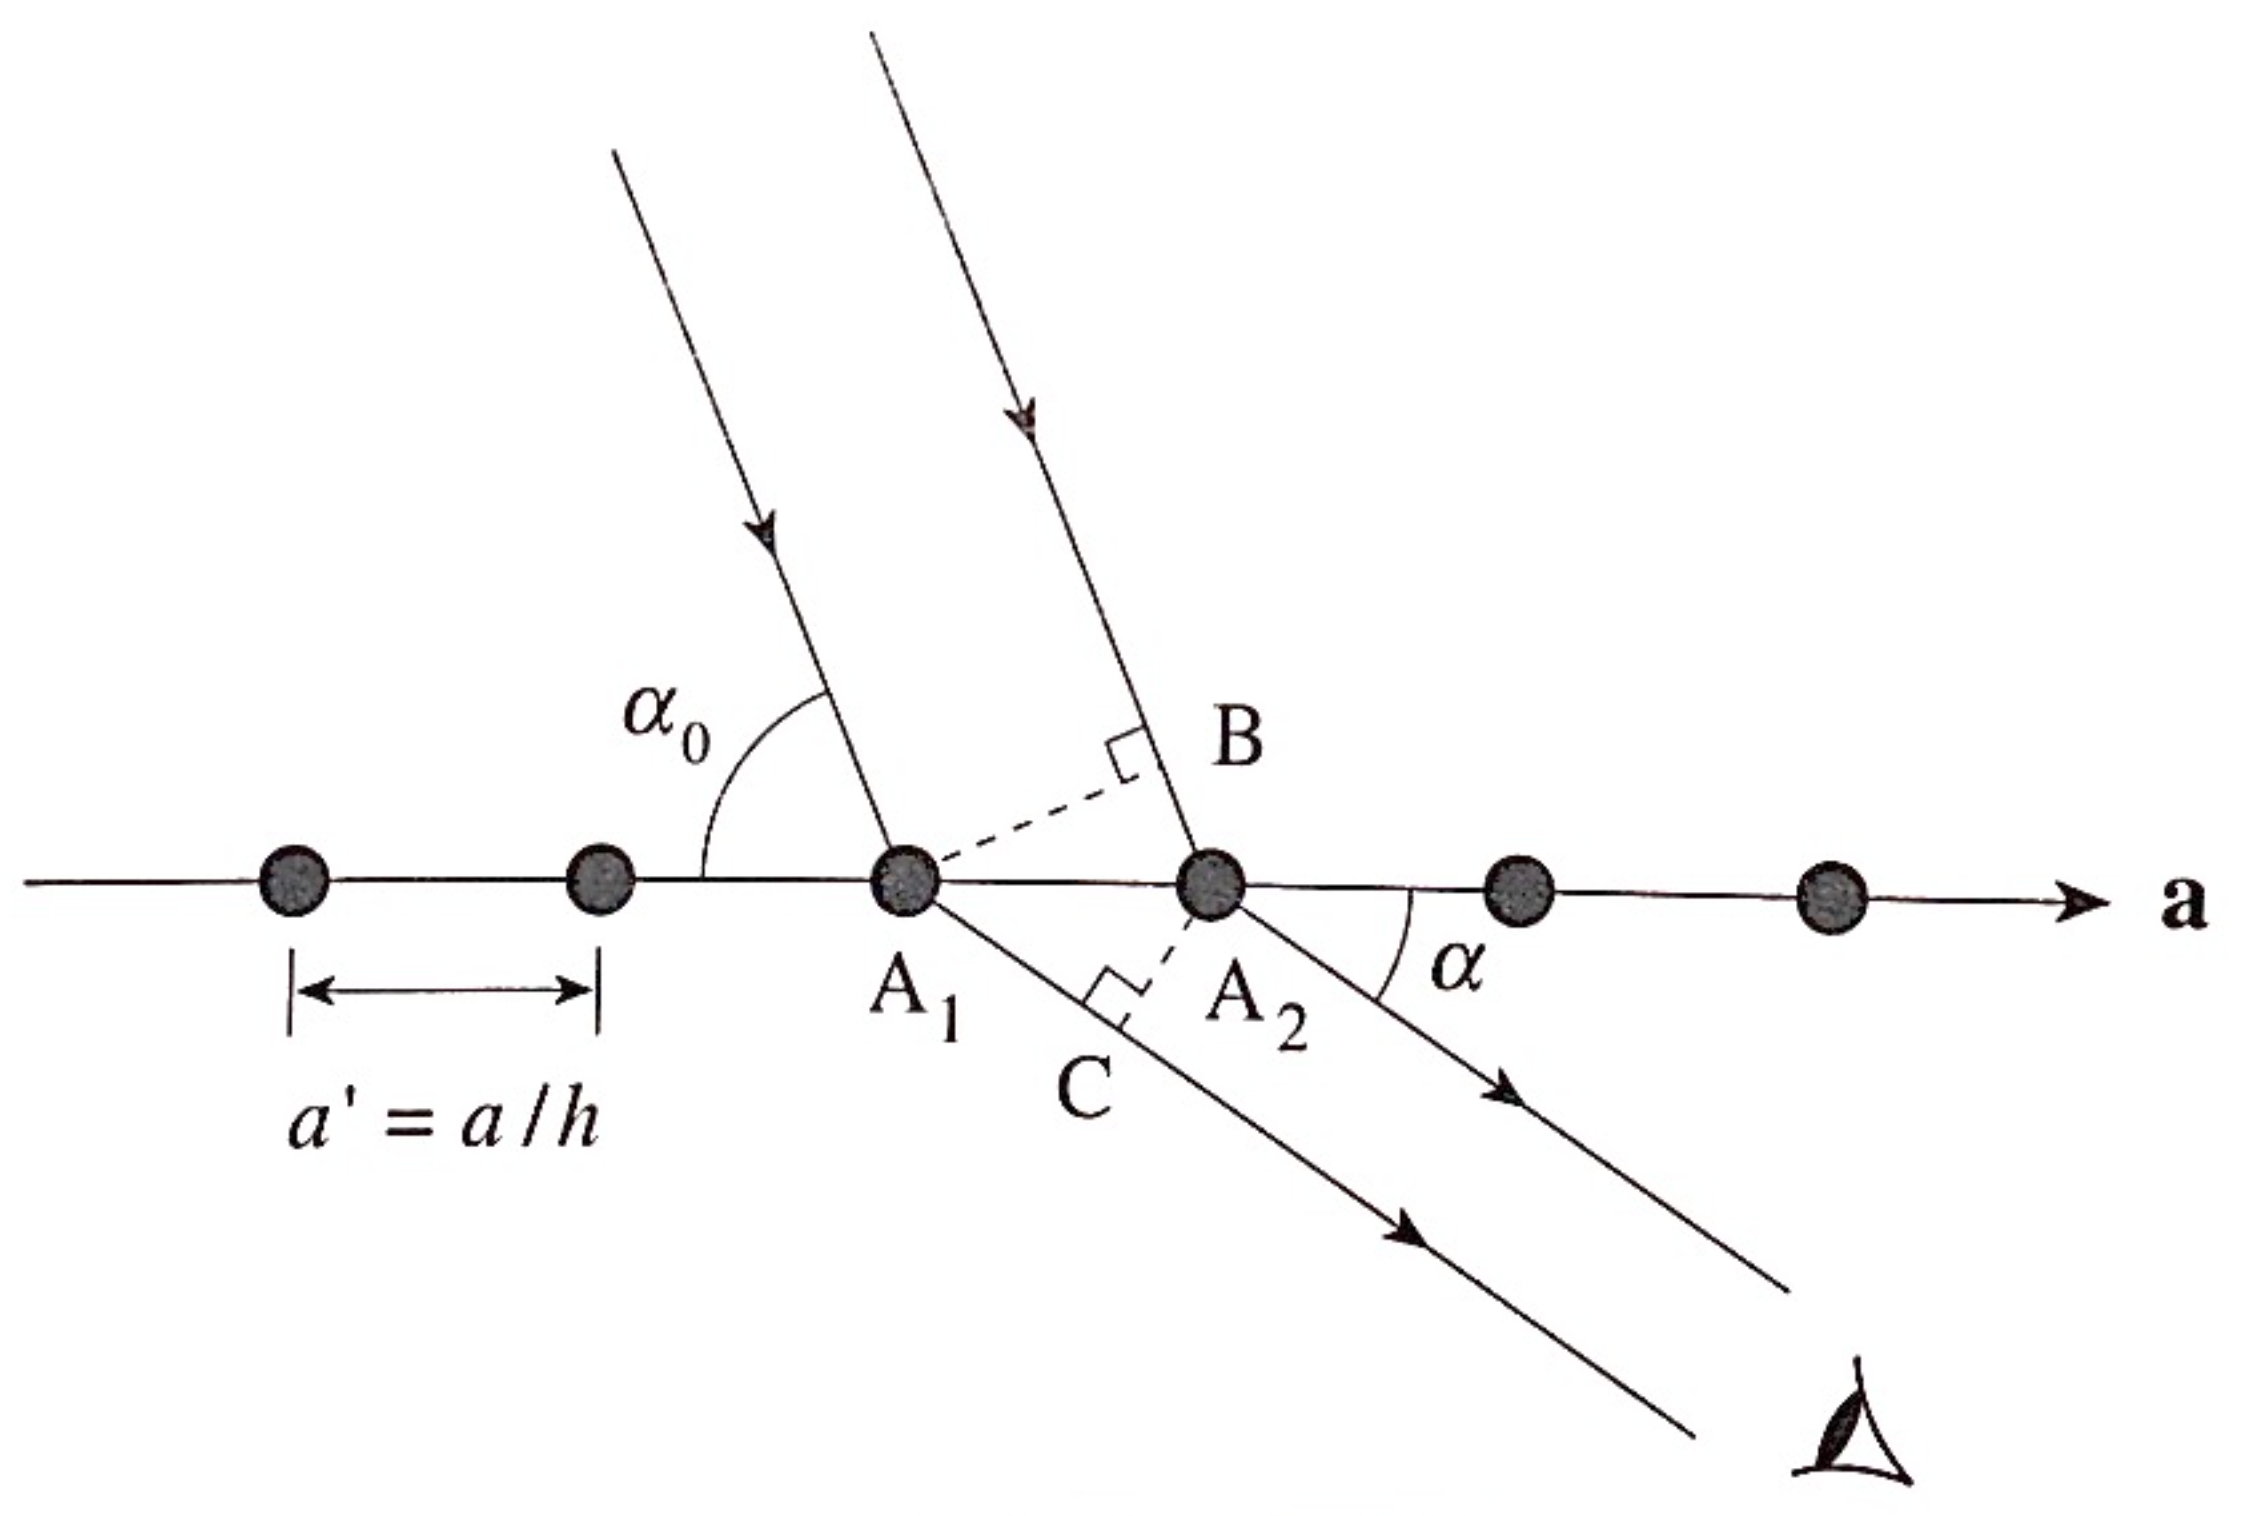
\includegraphics[width=0.45\linewidth]{../ExtFiles/vonLaueDerivation.png}
        \caption{Deriving the von Laue equations.}
        \label{fig:vonLaueDerivation}
    \end{figure}
    \begin{itemize}
        \item An X-ray diffraction pattern is a collection of spots of varying intensity.
        \begin{itemize}
            \item The arrangement of the spots provides a great deal of information on the crystal structure, as we will soon see.
        \end{itemize}
        \item We define
        \begin{equation*}
            \Delta = \overline{\text{A}_1\text{C}}-\overline{\text{A}_2\text{B}}
        \end{equation*}
        \begin{itemize}
            \item Imagine two parallel rays of light incident on points $\text{A}_1$ and $\text{A}_2$ in a crystal lattice.
            \item $\overline{\text{A}_1\text{C}}$ is the distance that the bottom beam travels after being scattered at $\text{A}_1$ and before the top beam is scattered at $\text{A}_2$.
            \item Symmetrically, $\overline{\text{A}_2\text{B}}$ is the distance that the top beam travels after the bottom beam is scattered at $\text{A}_2$ and before being scattered at $\text{A}_2$.
            \item Either way, $\Delta$ represents a kind of phase offset that occurs upon scattering. Say, for instance, that the two waves are in phase before scattering. Then from the perspective of the top wave, the bottom wave gets offset by $\Delta$ relative to it during the scattering process, and vice versa from the perspective of the bottom wave.
        \end{itemize}
        \item If the distance $\Delta$ is equal to an integral multiple of the wavelength of the X-ray radiation, the two diffracted beams will interfere constructively. Mathematically, since
        \begin{align*}
            \overline{\text{A}_1\text{C}} &= a'\cos\alpha&
            \overline{\text{A}_2\text{B}} &= a'\cos\alpha_0
        \end{align*}
        as we may readily read from Figure \ref{fig:vonLaueDerivation}, we require
        \begin{align*}
            n\lambda &= \Delta\\
            &= \overline{\text{A}_1\text{C}}-\overline{\text{A}_2\text{B}}\\
            &= a'(\cos\alpha-\cos\alpha_0)\\
            nh\lambda &= a(\cos\alpha-\cos\alpha_0)
        \end{align*}
    \end{itemize}
    \item \textbf{First-order reflection}: A diffraction spot that corresponds to $n=1$ in the above equation.
    \item \textbf{Second-order reflection}: A diffraction spot that corresponds to $n=2$ in the above equation.
    \item \textbf{$\bm{n}^\textbf{th}$-order reflection}: A diffraction spot that corresponds to $n$ in the above equation.
    \item \textbf{von Laue equations}: The following three equations, which relate the quantities involved in a first-order reflection. \emph{Given by}
    \begin{align*}
        a(\cos\alpha-\cos\alpha_0) &= h\lambda&
        b(\cos\beta-\cos\beta_0) &= k\lambda&
        c(\cos\gamma-\cos\gamma_0) &= l\lambda
    \end{align*}
    where $\alpha_0,\beta_0,\gamma_0$ are the angles of incidence of the X-ray radiation with respect to the \textbf{a}, \textbf{b}, and \textbf{c} axes of the crystal, respectively, and $\alpha$, $\beta$, and $\gamma$ are the corresponding diffraction angles.
    \item An example of how to use the von Laue equations.
    \begin{itemize}
        \item Consider the diffraction pattern obtained when an X-ray beam is directed at a crystal whose unit cell is primitive cubic.
        \item Orient the crystal such that the incident X-rays are perpendicular to the \textbf{a} axis of the crystal.
        \item Then the relevant von Laue equation reduces to $a\cos\alpha=h\lambda$.
        \item It follows that discrete angles will yield discrete spots?
    \end{itemize}
    \item A more general situation.
    \begin{itemize}
        \item For an arbitrary $hkl$ plane, the direction of diffraction with respect to the \textbf{a} axis is the same as that for the $h00$ planes. But there is also diffraction with respect to the \textbf{b} and \textbf{c} axes.
        \item The diffraction spots from an $hkl$ plane (with fixed $h$) will lie along the surface of a cone that makes an angle $\alpha$ with respect to the \textbf{a} axis of the crystal.
    \end{itemize}
    \item The Bragg diffraction.
    \begin{itemize}
        \item We have
        \begin{equation*}
            \lambda=2\left( \frac{d}{n} \right)\sin\theta
        \end{equation*}
        where $\theta$ is the angle of incidence (and reflection) of the X-rays with respect to the lattice plane, $\lambda$ is the wavelength of the X-ray radiation, and $n=1,2,\dots$ is the order of the reflection.
        \item $d$ in terms of the Miller indices for a cubic unit cell gives
        \begin{equation*}
            \sin^2\theta = \frac{n^2\lambda^2}{4a^2}(h^2+k^2+l^2)
        \end{equation*}
        \item Tian will not go through the details, but there will be a homework problem in which we will explore this.
    \end{itemize}
    \item Rotating the sample vs. rotating the incident beam in an X-ray diffraction experiment.
    \begin{itemize}
        \item In most cases, we fix the incident beam orientation and rotate the sample on the sample stage.
    \end{itemize}
    \item Midterms back today or tmw.
    \item The grade distribution in the course.
    \begin{itemize}
        \item A or A- is typically 65-70\%.
    \end{itemize}
\end{itemize}



\section{The Scattering Factor and Intensity}
\begin{itemize}
    \item \marginnote{5/18:}Reviews the Bragg diffraction.
    \begin{itemize}
        \item There is no such thing as a 222 or a 333 lattice plane; rather, there are 111 lattice planes with higher order diffractions.
        \item Tian says something about higher order reflections?
    \end{itemize}
    \item \textbf{Scattering factor} (of an atom): The following quantity, where $\rho(r)$ is the spherically symmetric electron density (number of electrons per unit volume) of the atom and $k=4\pi\sin(\theta)/\lambda$. In turn, $\theta$ is the scattering angle and $\lambda$ is the wavelength of the X-radiation. \emph{Denoted by} $\bm{f}$. \emph{Given by}
    \begin{equation*}
        f = 4\pi\int_0^\infty\rho(r)\frac{\sin kr}{kr}r^2\dd{r}
    \end{equation*}
    \begin{itemize}
        \item The integral $4\pi\int_0^\infty\rho(r)r^2\dd{r}$ gives the total number of electrons in the atom.
    \end{itemize}
    \item The total scattering intensity is related to the periodic structure of the electron density in the crystal.
    \begin{itemize}
        \item If the crystal is oriented such that the von Laue equation governing scattering from atoms along the $a$ axis is satisfied, then
        \begin{align*}
            \Delta_{11} &= \Delta_{22}
                = \frac{a}{h}(\cos\alpha-\cos\alpha_0)
                = \lambda&
            \Delta_{12} &= x(\cos\alpha-\cos\alpha_0)
        \end{align*}
        \item Combining these two equations, we learn that
        \begin{equation*}
            \Delta_{12} = \frac{\lambda hx}{a}
        \end{equation*}
        \item The difference in path length corresponds to a phase difference between the diffracted beams from successive 1 and 2 atoms of
        \begin{equation*}
            \phi = 2\pi\frac{\Delta_{12}}{\lambda}
            = 2\pi\frac{\lambda hx/a}{\lambda}
            = \frac{2\pi hx}{a}
        \end{equation*}
        \item The amplitude of the light scattered from successive 1 and 2 atoms is then
        \begin{align*}
            A &= f_1\cos\omega t+f_2\cos(\omega t+\phi)\\
            &= f_1\e[i\omega t]+f_2\e[i(\omega t+\phi)]
        \end{align*}
        \item The detected intensity is proportional to the square of the magnitude of the amplitude.
        \begin{align*}
            I \propto |A|^2 &= [f_1\e[i\omega t]+f_2\e[i(\omega t+\phi)]][f_1\e[-i\omega t]+f_2\e[-i(\omega t+\phi)]]\\
            &= f_1^2+f_1f_2\e[i\phi]+f_1f_2\e[-i\phi]+f_2^2\\
            &= f_1^2+f_2^2+2f_1f_2\cos\phi
        \end{align*}
        \begin{itemize}
            \item The first two terms reflect the constructive interference of the X-rays scattered from the set of parallel planes through the 1 atoms and 2 atoms, respectively.
            \item The third term takes into account the interference of the scattering from these two sets of parallel planes.
        \end{itemize}
        \item We can therefore ignore the $\e[i\omega t]$ term and define
        \begin{equation*}
            F(h) = f_1+f_2\e[i\phi]
            = f_1+f_2\e[2\pi ihx/a]
        \end{equation*}
        \item The intensity is then proportional to $|F(h)|^2$.
        \item Generalizing to three dimensions for a unit cell that contains atoms of type $j$ located at points $x_j,y_j,z_j$ gives
        \begin{equation*}
            F(hkl) = \sum_jf_j\e[2\pi i(hx_j/a+ky_j/b+lz_j/c)]
            = \sum_jf_j\e[2\pi i(hx_j'+ky_j'+lz_j')]
        \end{equation*}
        where $x_j'=x_j/a$, $y_j'=y_j/b$, and $z_j'=z_j/c$.
    \end{itemize}
    \item An analysis of the \ce{CsCl} body-centered cubic lattice, where we take the unit cell to have eighth chloride atoms at every corner and one cesium ion in the center.
    \begin{itemize}
        \item Taking $f_+$ to be the scattering factor of the \ce{Cs+} cations and $f_-$ to be the scattering factor of the \ce{Cl-} anions, we get
        \begin{align*}
            F(hkl) &= 1\times f_-\e[\pi i(h+k+l)]+\frac{1}{8}\times f_+\left[ \e[0]+\e[2\pi ih]+\e[2\pi ik]+\e[2\pi il]+\e[2\pi i(h+k)]+\e[2\pi i(k+l)]+\e[2\pi i(h+l)]+\e[2\pi i(h+k+l)] \right]\\
            &= f_-(-1)^{h+k+l}+\frac{1}{8}f_+[8]\\
            &=
            \begin{cases}
                f_++f_- & h+k+l\text{ is even}\\
                f_+-f_- & h+k+l\text{ is odd}
            \end{cases}
        \end{align*}
        where we substitute $\e[\pi i]=-1$ and $\e[2\pi i]=1$ to get from the first line to the second.
    \end{itemize}
\end{itemize}



\section{Continuous Structure Factors and Adsorption}
\begin{itemize}
    \item \marginnote{5/20:}More on the \ce{CsCl} example today.
    \begin{itemize}
        \item We simplify $\e[i\pi(h+k+l)]$ to $(-1)^{h+k+l}$ by expanding to $\cis[\pi(h+k+l)]$, ignoring the imaginary part to get $\cos[\pi(h+k+l)]$, the sign of which does depend on whether the natural number $h+k+l$ is even or odd exactly like $(-1)^{h+k+l}$.
    \end{itemize}
    \item \ce{CsI} example.
    \begin{itemize}
        \item \ce{Cs+} and \ce{I-} are \textbf{isoelectronic}.
        \item We have that
        \begin{equation*}
            f_+(\ce{Cs+}) = f_-(\ce{I-})
        \end{equation*}
    \end{itemize}
    \item The structure factor and the electron density are related by a Fourier transform.
    \begin{itemize}
        \item In both atomic and molecular crystals, the electron density is not localized at individual points within the unit cell.
        \item We should consider the unit cell of the crystal to have a continuous electron density distribution $\rho(x,y,z)$.
        \item The structure factor is no longer simply a sum over discrete atoms but now becomes an integral over the continuous electron density distribution in the unit cell, as follows.
        \begin{equation*}
            F(hkl) = \int_0^a\int_0^b\int_0^c\rho(x,y,z)\e[2\pi i(hx/a+ky/b+lz/c)]\dd{x}\dd{y}\dd{z}
        \end{equation*}
        \item For the entire crystal, we have the following.
        \begin{equation*}
            F(hkl) \propto \int_{-\infty}^\infty\int_{-\infty}^\infty\int_{-\infty}^\infty\rho(x,y,z)\e[2\pi i(hx/a+ky/b+lz/c)]\dd{x}\dd{y}\dd{z}
        \end{equation*}
        \item $F(hkl)$ is related to $\rho(x,y,z)$ by a \textbf{Fourier transform}.
        \begin{equation*}
            \rho(x,y,z) = \sum_{h=-\infty}^\infty\sum_{k=-\infty}^\infty\sum_{l=-\infty}^\infty F(hkl)\e[-2\pi i(hx/a+ky/b+lz/c)]
        \end{equation*}
        \item If we let $F(hkl)=A(hkl)+iB(hkl)$, then it follows that the intensity is
        \begin{equation*}
            I(hkl) \propto |F(hkl)|^2 = [A(hkl)]^2+[B(hkl)]^2
        \end{equation*}
    \end{itemize}
    \item An electron-density map of a benzoic acid molecule.
    \begin{figure}[h!]
        \centering
        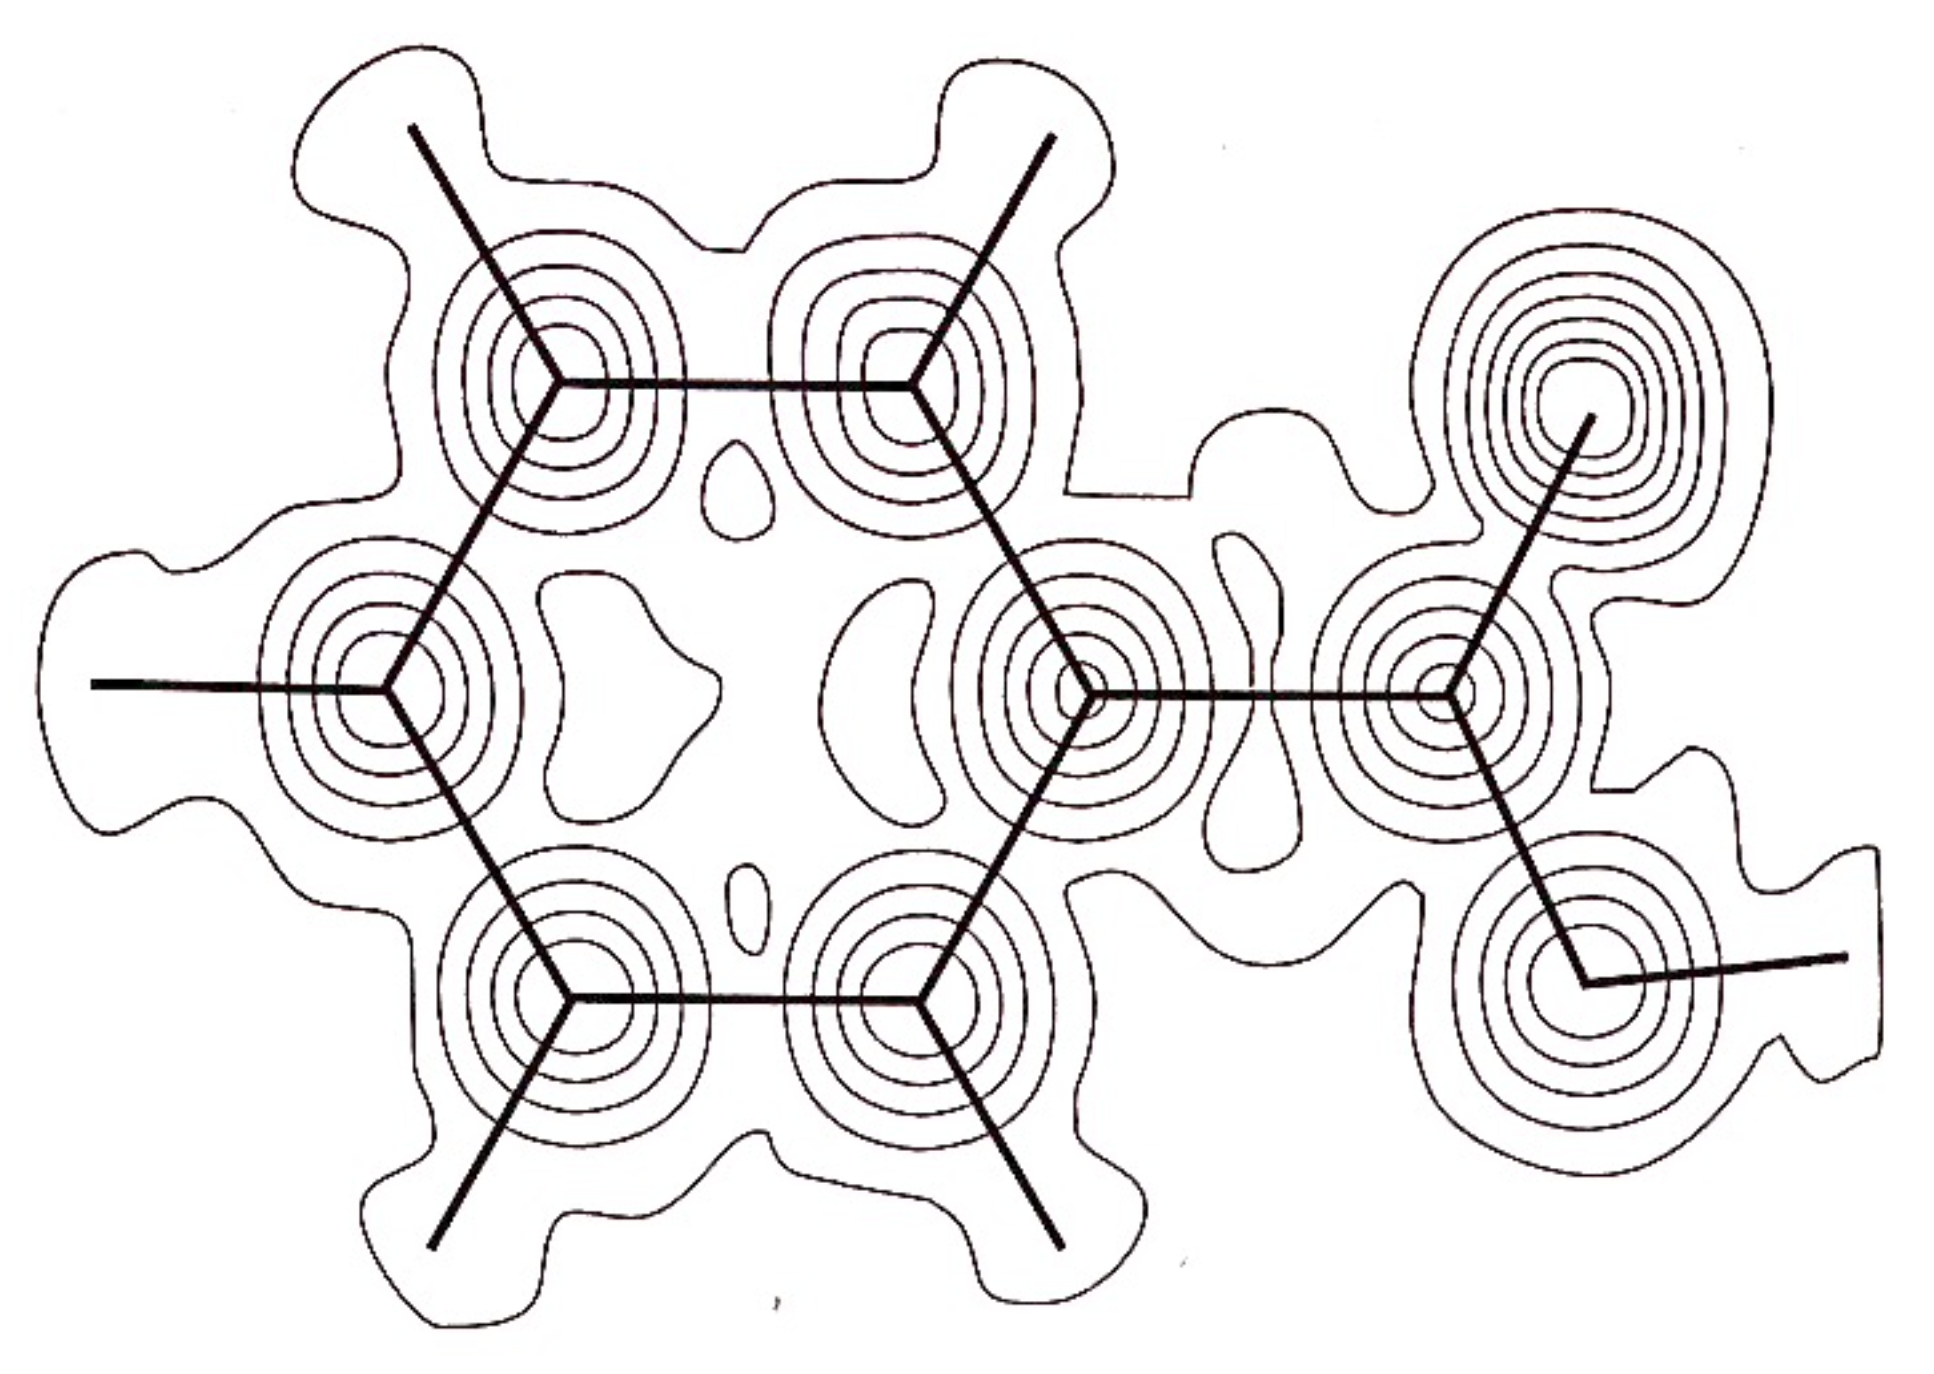
\includegraphics[width=0.4\linewidth]{../ExtFiles/benzoicAcidEdensity.png}
        \caption{The electron density of benzoic acid.}
        \label{fig:benzoicAcidEdensity}
    \end{figure}
    \begin{itemize}
        \item An electron-density map of a benzoic acid molecule determined from the X-ray diffraction pattern of a benzoic acid crystal.
        \item Each contour line corresponds to a constant value of the electron density.
        \item The location of the nuclei are readily deduced from this electron-density map and are represented by the vertices of the solid lines.
    \end{itemize}
    \item A gas molecule can physisorb or chemisorb to a solid surface.
    \begin{figure}[h!]
        \centering
        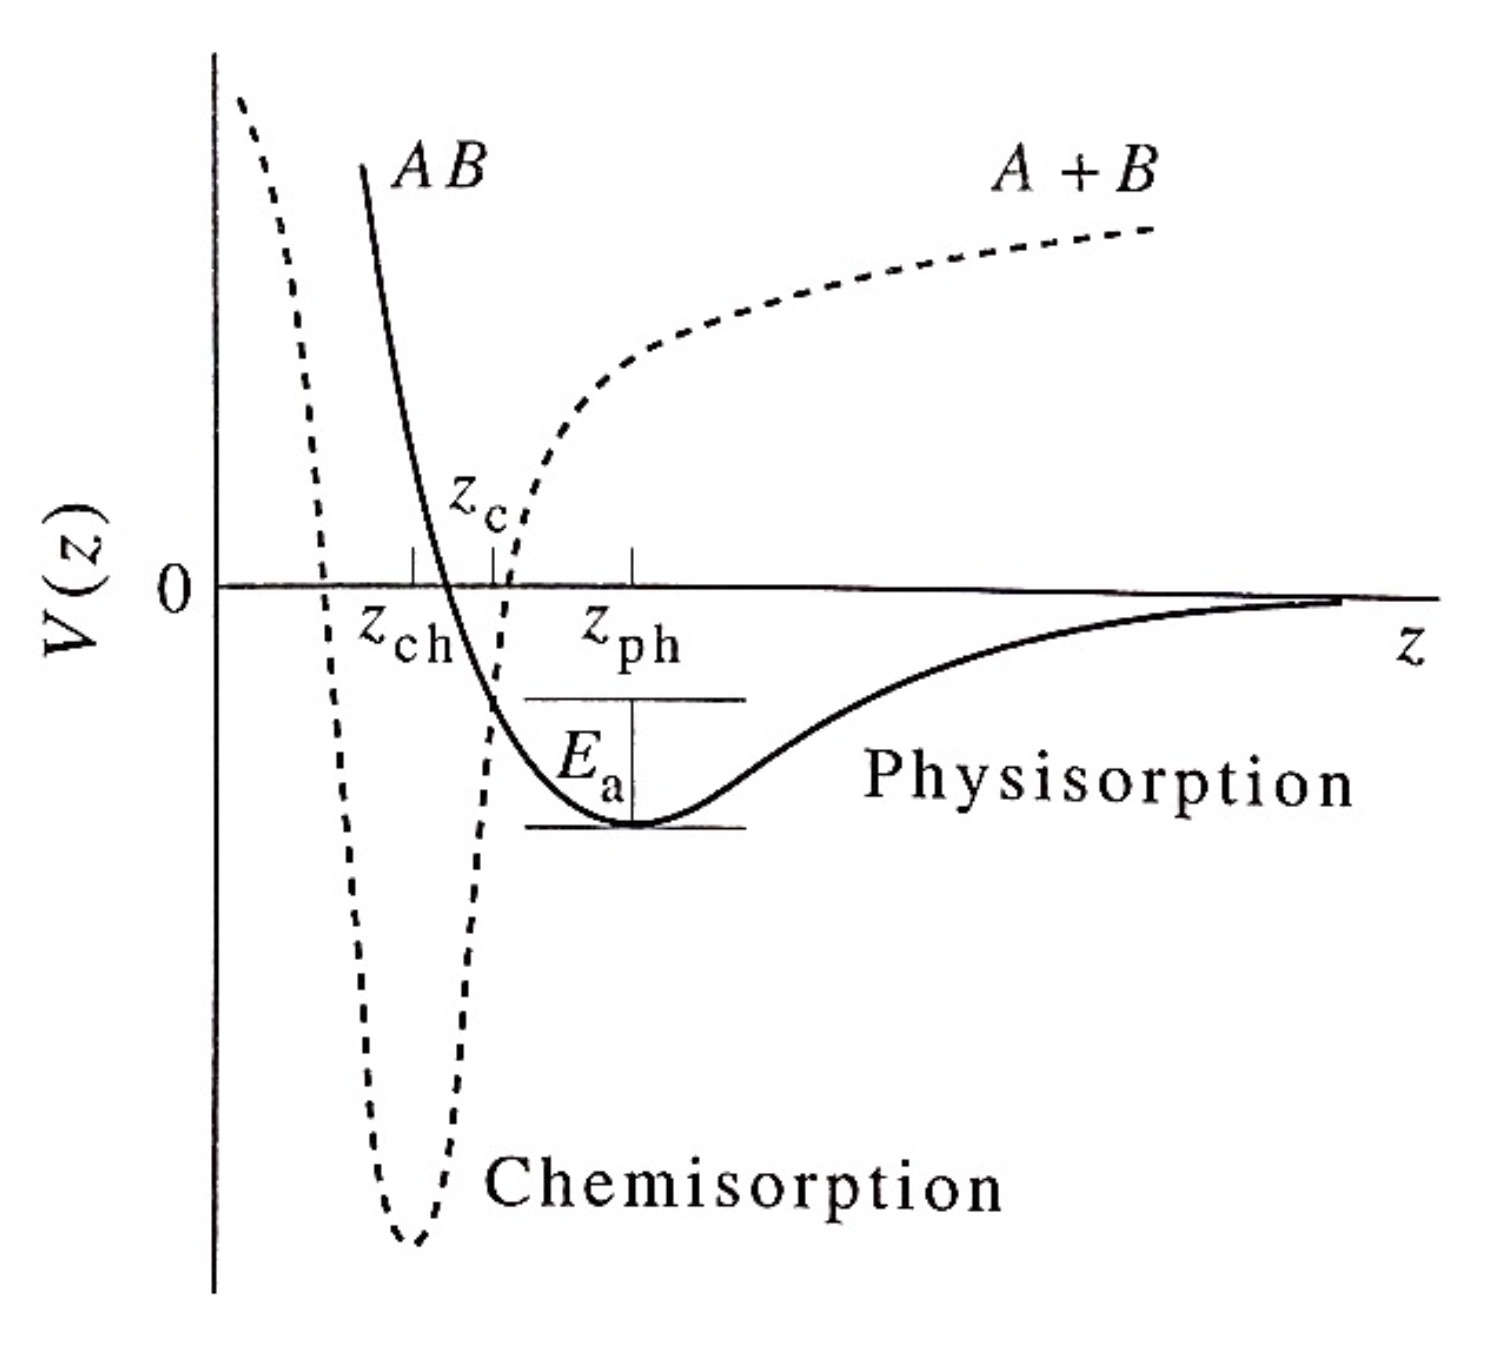
\includegraphics[width=0.36\linewidth]{../ExtFiles/PhysiChemiSorption.png}
        \caption{Comparing physisorption and chemisorption.}
        \label{fig:PhysiChemiSorption}
    \end{figure}
    \begin{itemize}
        \item Figure \ref{fig:PhysiChemiSorption} shows one-dimensional potential-energy curves for the physisorption of molecule \ce{AB} (solid line) and the dissociative chemisorption of \ce{AB} (dashed line).
        \item The quantity $z$ is the distance from the surface.
        \item In the physisorbed state, the molecule \ce{AB} is bound to the surface by van der Waals forces.
        \item In the chemisorbed state, the \ce{A-B} bond is broken, and the individual atoms are bound covalently or ionically on the surface.
        \begin{itemize}
            \item As such, chemisorbed molecules are bound more strongly, are held closer to the surface.
            \item As $z\to\infty$, $V$ approaches a value greater than zero because \ce{AB} is dissociated here. The asymptote is the bond dissociation energy (BDE).
            \item Additionally, while \ce{A + B} may be at zero, what we have here is \ce{A+ + B-}. As such, we have the Coulomb potential, and the charged ions are unstable to be apart.
        \end{itemize}
        \item The points $z_\text{ch}$ and $z_\text{ph}$ are the surface-molecule bond lengths for a chemisorbed and physisorbed molecule, respectively. The length of the substrate-adsorbate bond is shorter for a chemisorbed molecule than for a physisorbed molecule.
        \item The two potential curves cross at $z_c$. The activation energy for the conversion from physisorption to chemisorption is measured from the bottom of the physisorbed potential and is $E_a$.
    \end{itemize}
    \item \textbf{Adsorption isotherm}: A plot of surface coverage as a function of gas pressure at constant temperature.
    \item Langmuir's assumptions.
    \begin{itemize}
        \item The adsorbed molecules do not interact with one another.
        \item The enthalpy of adsorption was independent of surface coverage.
        \item There are a finite number of surface sites where a molecule can adsorb.
        \item The process of adsorption and desorption is depicted by the reversible elementary process
        \begin{equation*}
            \ce{A(g) + S(s)} \Longleftrightarrows[k_a][k_d] \ce{A-S(s)}
        \end{equation*}
        with equilibrium constant
        \begin{equation*}
            K_c = \frac{k_a}{k_d}
            = \frac{\cnc{A-S}}{\cnc{A}\cnc{S}}
        \end{equation*}
        where $k_a$ and $k_d$ are the rate constants for \underline{a}dsorption and \underline{d}esorption, respectively.
    \end{itemize}
    \item The fact that $k_a$ and $k_d$ are constants independent of the extent of surface coverage implies that adsorbed molecules do not interact with one another.
    \item An analysis of surface coverage.
    \begin{itemize}
        \item Let $\sigma_0$ be the concentration of surface sites in units of \si{\per\meter\squared}.
        \item If the fraction of surface sites occupied by an adsorbate is $\theta$, then $\sigma$ (the adsorbate concentration on the surface) is $\theta\sigma_0$ and the concentration of empty surface sites is give by $\sigma_0-\theta\sigma_0=(1-\theta)\sigma_0$.
        \item We have that
        \begin{align*}
            v_d &= k_d\theta\sigma_0&
            v_a &= k_a(1-\theta)\sigma_0\cnc{A}
        \end{align*}
        where $v_d$ is the rate of desorption, $v_a$ is the rate of absorption, and $\cnc{A}$ is the number density or the concentration of \ce{A(g)}.
        \item It follows that at equilibrium,
        \begin{align*}
            k_d\theta &= k_a(1-\theta)\cnc{A}\\
            \frac{1}{\theta} &= 1+\frac{1}{K_c\cnc{A}}
        \end{align*}
        \item Additionally, since
        \begin{align*}
            \cnc{A} = \frac{P_{\ce{A}}}{\kB T}
        \end{align*}
        the Langmuir adsorption isotherm is
        \begin{equation*}
            \frac{1}{\theta} = 1+\frac{1}{bP_{\ce{A}}}
        \end{equation*}
        where we have defined $b=K_c/\kB T$.
    \end{itemize}
    \item For different materials, the same mass may correspond to orders of magnitude different surface areas (consider MOFs for instance).
    \item Langmuir adsorption isotherm for the case in which a diatomic molecule dissociates upon adsorption to the surface.
    \begin{itemize}
        \item This reaction can be written as
        \begin{align*}
            \ce{A2(g) + 2S(s)} &\Longleftrightarrows[k_a][k_d] \ce{2A-S(s)}&
            K_c &= \frac{k_a}{k_d}
                = \frac{\cnc{A-S}^2}{\cnc{A2}\cnc{S}^2}
        \end{align*}
        \item Two surface sites are involved in the adsorption and desorption process.
        \begin{align*}
            v_a &= k_a\cnc{A2}(1-\theta)^2\sigma_0^2&
            v_d &= k_d\theta^2\sigma_0^2
        \end{align*}
        \item At equilibrium, these rates are equal, i.e.,
        \begin{align*}
            k_a\cnc{A2}(1-\theta)^2 &= k_d\theta^2\\
            \theta &= \frac{K_c^{1/2}\cnc{A2}^{1/2}}{1+K_c^{1/2}\cnc{A2}^{1/2}}
        \end{align*}
        \item Having defined $\cnc{A}=P_{\ce{A}}/\kB T$ and $b=K_c/\kB T$, we have
        \begin{align*}
            \theta &= \frac{b_{\ce{A2}}^{1/2}P_{\ce{A2}}^{1/2}}{1+b_{\ce{A2}}^{1/2}P_{\ce{A2}}^{1/2}}\\
            \frac{1}{\theta} &= 1+\frac{1}{b_{\ce{A2}}^{1/2}P_{\ce{A2}}^{1/2}}
        \end{align*}
    \end{itemize}
\end{itemize}



\section{Office Hours (Tian)}
\begin{itemize}
    \item The whole $F\propto\sigma\rho$ thing from Lecture 4.
    \item The presence of lack thereof of the $1/2$ coefficient in $Z_{\ce{A}\ce{A}}$ and $Z_{\ce{A}\ce{B}}$.
    \item Lecture 13 example problems.
    \begin{itemize}
        \item Equilibrium constants appear in reversible reactions.
        \item Only applicable for reversible elementary steps.
        \item If there's a problem that involves equilibrium constants, he will identify it; tell us that a reaction is reversible and equilibrium constants need to be considered.
    \end{itemize}
    \item Will there be extra office hours before the final?
    \item Midterm info.
    \begin{itemize}
        \item The midterm had a bimodal (2 peaks) distribution.
    \end{itemize}
    \item Miller indices.
    \begin{itemize}
        \item We define 100 planes by convention.
        \item The middle plane in Figure 31.9a intersects the $a$-axis at $(1,0,0)$, and never intersects the $b$ or $c$ axes. However, we can conceptually define an intersection at $\infty$, leading to $k=b/\infty=0$ and similarly for $l$.
    \end{itemize}
    \item Final info.
    \begin{itemize}
        \item Homeworks 5-6 for the computation problem.
        \item Rest are true/false and conceptual (like defining the Miller indices, for example).
        \item Open note, calculator, but not open internet.
        \item We can bring our computer for online notes, but we cannot search anything.
        \item Only conceptual problems on X-ray diffraction.
        \item No class on Friday Week 9.
    \end{itemize}
    \item X-ray diffraction info.
    \begin{itemize}
        \item Some people who have taken Advanced Inorgo will have already seen this, but it's the first time for most people.
    \end{itemize}
\end{itemize}




\end{document}